\documentclass[14pt, fleqn, xcolor={dvipsnames, table}]{beamer}
\usepackage[T2A]{fontenc}
\usepackage[utf8]{inputenc}
\usepackage[english,russian]{babel}
\usepackage{amssymb,amsfonts,amsmath,mathtext}
\usepackage{cite,enumerate,float,indentfirst}
\usepackage{cancel}

\usepackage{tikz}                   
\usetikzlibrary{shadows}

% \usepackage{enumitem}
% \setitemize{label=\usebeamerfont*{itemize item}%
%   \usebeamercolor[fg]{itemize item}
%   \usebeamertemplate{itemize item}}

\graphicspath{{images/}}

\usetheme{Madrid}
\usecolortheme{seahorse}
\renewcommand{\CancelColor}{\color{red}}

\setbeamercolor{footline}{fg=Blue!50}
\setbeamertemplate{footline}{
  \leavevmode%
  \hbox{%
  \begin{beamercolorbox}[wd=.333333\paperwidth,ht=2.25ex,dp=1ex,center]{}%
    И. Кураленок, Н. Поваров, Яндекс
  \end{beamercolorbox}%
  \begin{beamercolorbox}[wd=.333333\paperwidth,ht=2.25ex,dp=1ex,center]{}%
    Санкт-Петербург, 2013
  \end{beamercolorbox}%
  \begin{beamercolorbox}[wd=.333333\paperwidth,ht=2.25ex,dp=1ex,right]{}%
  Стр. \insertframenumber{} из \inserttotalframenumber \hspace*{2ex}
  \end{beamercolorbox}}%
  \vskip0pt%
}
\newcommand\indentdisplays[1]{%
     \everydisplay{\addtolength\displayindent{#1}%
     \addtolength\displaywidth{-#1}}}
\newcommand{\itemi}{\item[\checkmark]}

\title{Линейные модели: SVM (продолжение). Collaborative filtering.\\\small{}}
\author[]{\small{%
И.~Куралёнок,
Н.~Поваров}}
\date{}

\begin{document}

\begin{frame}

\maketitle
\small
\begin{center}
\vspace{-60pt}
\normalsize {\color{red}Я}ндекс \\
\vspace{80pt}
\footnotesize СПб, 2013
\end{center}
\end{frame}

% Классные слайды http://www.cs.nyu.edu/~mohri/icml2011-tutorial/tutorial-icml2011-1.pdf
\section{SVM (продолжение)}
\begin{frame}{Что мы узнали в прошлый раз}
\small
\begin{itemize}
  \item Было бы классно найти такую плоскость, которая сильнее всего поделит на классы
  \item Если множества линейно разделимы, то надо минимизировать $\|w\|$
  \item Если перейти к дуальной задаче, зависимость от $x$ окажется только через скалярные произведения, которые мы можем ``организовать'' по своему разумению
  \item В дуальном решении условия очень просты и можно организовать безусловную оптимизацию заменой переменных
  \item Количество компонент оптимизации пропорционально квадрату количества точек, что много
\end{itemize}
\end{frame}

\subsection{SVM в случае неразделимых множеств} % из вики

\begin{frame}{Мягкие границы}
\begin{center}
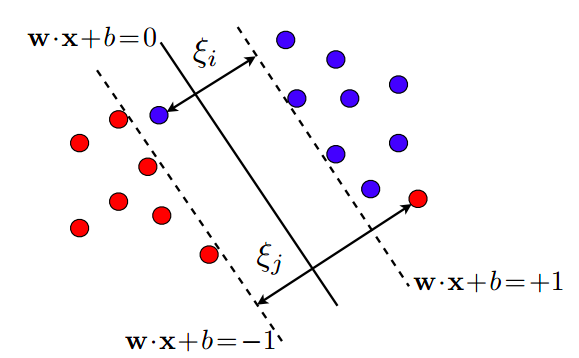
\includegraphics[height=0.4\textheight]{SoftMargins.png}
\end{center}
Перенесем точки-``нарушители'' на границу и добавим к целевой функции стоимость этого переноса:
$$\begin{array}{l}
\arg \min \|w\| + c\sum_i \xi_i \\
\left\{\begin{array}{l}
y_i(\beta^T x_i - b) + \xi_i \ge 1 \\
\xi_i \ge 0
\end{array}\right.
\end{array}$$
\end{frame}

\begin{frame}{Решение с мягкими границами}
\small
Прямая задача:
$$\begin{array}{ll}
\arg \min_{w,\xi,b} \max_{\lambda} & \|w\| \\
  & + c\sum_i \xi_i \\
  & - \sum_i \lambda_{i} \left(y_i (w x_i - b) + \xi_i - 1\right) \\
  & - \sum_i \lambda_{i+n} \xi_i \\
\lambda_i > 0
\end{array}$$

Дуальная задача (Wolfe):
$$
\begin{array}{l}  
\arg \max_{\lambda} \sum_{i=1}^m\lambda_i - \frac{1}{2}\sum_{i=1}^m\sum_{j=1}^m\lambda_i\lambda_j y_i y_j (x_i x_j) \\  

\left\{\begin{array}{ll}  
  0 \le \lambda_i \le c & \\
  \sum_{i=1}^m\lambda_i y_i = 0
  \end{array}   
\right.
\end{array}
$$
Где-то мы такое уже видели.
\end{frame}

\begin{frame}{Нелинейные решения в SVM (Ядра)}
\small
Построим преобразование из исходного пространтсва в какое-то евклидово $\mathcal{H}$:
$$
\Phi: \mathbb{R}^n \to \mathcal{H}
$$
Тогда определим $(x_i, x_j) = (\Phi(x_i), \Phi(x_j))$. Что можно делать с ядрами \footnote{доказывается либо через определение, либо через теорему Мерцера}:
\begin{enumerate}
\footnotesize
  \item линейно комбинировать
  \item умножать
  \item комбинировать с функцией, раскладываемой в Тейлора с неотрицательными коэффициентами (например $e^x$)
  \item etc.
\end{enumerate}
В задаче можно поставить цель подобрать оптимальное ядро с помощью подобных преобразований.
\end{frame}

\begin{frame}{Известные Ядра}
\small
\begin{description}
  \item[Полиномиальные] $K(x,x^{'}) = (x^Tx^{'} + c)^d$ 
  \item[Гауссово (radial basis)] $K(x,x^{'}) = e^{-\gamma \|x - x^{'}\|_2^2}$ 
  \item[Сигмойдное (``Нейронное'')] $K(x,x^{'}) = tanh(k_1 (x,x^{'}) + k_2)$ 
\end{description}
В этом случае решение будет выглядеть иначе:
$$
h(x) = sign \left(\sum_i \lambda_i y_i (K(x_i, x) + b)\right)
$$
Заметим, что можно выкинуть все точки в которых $\lambda_i = 0$ (это какие?).
\end{frame}

\subsection{Сведение SVM к линейной системе с регуляризацией} % из книжки

\begin{frame}{SVM и регуляризация}
\small
Вспомним как выглядит наша решающая функция (без ядер): $h(x) = sign(x^T w + b)$. Тогда проблему можно переформулировать так:
$$
\min \sum_i (1 - y_i h(x_i))_+ + \frac{\lambda}{2} \|w\|^2
$$
А это минимизация hinge loss с $l_2$ регуляризацией. Теперь тоже самое, но с ядрами, $h(x) = sign \left(\sum_i \lambda_i y_i (K(x_i, x) + b)\right)$:
$$
\min \sum_i (1 - y_i h(x_i))_+ + \frac{\lambda}{2} w^T K w
$$
где $K : k_{ij} = K(x_i, x_j)$. Нас никто не ограничивает hinge loss, можно все тоже самое, но с любым другим лосем!
\end{frame}

\begin{frame}{Kernel Ridge Regression}
\small
Если применима к любым функциям потерь, то почему не к $l_q$? Нормировка $b$ нам теперь не нужна, поэтому:
$$
h(x) = sign \left(\sum_i \lambda_i K(x_i, x)\right)
$$
Поигравшись в подстановку получим:
$$
\min_\lambda с \lambda^T\lambda - 2 \lambda y - \lambda^T K \lambda
$$
или
$$
\min_\lambda \lambda (K + cE) \lambda - 2\lambda^T y
$$
или
$$
\lambda = \left(K + с E\right)^{-1}y
$$
\end{frame}

%\subsection{Простая оптимизация SVM} % ? из головы /machinelearning.ru
\section{Построение мультиклассификатора} % best 10 years paper award ICML2010
\begin{frame}{Как построить мультиклассификатор?}
\begin{itemize}
  \item Выберем очки для каждого класса и сведем задачу к регрессии
  \item Один против всех в количестве $k$ штук
  \item Построим одновременно несколько классификаторов с условием их соотношения (Multi-logit)
  \item Построим классификаторы для всех пар
  \item Есть еще идеи?
\end{itemize}
\end{frame}

\begin{frame}{Reducing multiclass to binary}
\small
E.L.~Allwien, R.E.~Schapire, Y.~Singer предложили интересную альтернативу:
Введем модельную матрицу $\mathcal{M} \in \{-1,0,1\}^{k\times l}$. Для каждого столбца подберем функцию бинарной классификации, отделяющую $+1$ от $-1$.
Решим исходную задачу одним из двух способов:
$$
d_H(c, f(x), \mathcal{M}) = \sum_{s = 1}^l\left({1 - sign(m_{cs} f_s(x)) \over 2}\right)
$$
$$
d_L(c, f(x), \mathcal{M}) = \sum_{s = 1}^l L(m_{cs} f_s(x))
$$
Теперь вопрос свелся к тому как найти оптимальный $\mathcal{M}$.
\end{frame}

\section{Collaborative filtering}

\subsection{Пример} % переработать http://habrahabr.ru/company/surfingbird/blog/139022/ на Сифона/Бороду
% \begin{frame}{Вася и Петя \& подарки}
% Вася и Петя собирали подарки для друзей из другого города. Друзья загадочные, но известно, что у них есть. Надо подобрать подарки так, чтобы им понравилось, используя знание о том, что обычно встречается вместе в домах.
% \end{frame}

\subsection{Постановка задачи} % wiki
\begin{frame}{Collaborative filtering}
Есть пользователи, есть товары. Надо найти подходящие пользователю товары, которых он не видел, используя информацию о том какие товары покупают вместе.
$$\begin{array}{l}
U = \{u_i\}_1^n, R = \{r_j\}_1^m \\
X = \{(u, r, s) | u \in U, r \in R, s \in \mathbb{Z}_S \}
\end{array}$$
{\color{blue}www.netflixprize.com} проводит соревнование с призом в 1m\$. $n \simeq 480k, m \simeq 17k$.
$$
L(h, X) = -\sum_{(u,r,s) \in X} \|s - h(r,s)\|_2
$$
\end{frame}

\begin{frame}{Принципиальные способы решения}
\begin{itemize}
  \item Храним весь опыт в памяти:
  \begin{description}
    \item[\color{green}+] просто, можно легко обновлять;
    \item[\color{red}---] может быть тяжело по памяти, возможен только простой анализ, так как все работает on the fly.
  \end{description}
  \item Храним только профайлы для пользователей и товаров:
  \begin{description}
    \item[\color{green}+] легко шардируется, менее требовательно по памяти;
    \item[\color{red}---] сложнее обновлять, для высокой отзывчивости надо городить охретектуру.
  \end{description}
\end{itemize}
\end{frame}

\subsection{Случай, когда матрица полная} % Воронцов, лекция в ВШЭ http://www.machinelearning.ru/wiki/images/e/e5/Voron-2008-11-10-cf.pdf

\begin{frame}{Потоварные методы: линейная регрессия}
Если есть звезды, то можно сделать все просто:
$$
h(u, r|X) = \sum_{\footnotesize\begin{array}{c}(u,q,s) \in X \\ q \ne r\end{array}} a_q s + b_q
$$
Slope One:
$$
h(u, r|X) = \frac{1}{\sum_{q \ne r} |X(r,q)|} \sum_{\footnotesize\begin{array}{c}(u,q,s) \in X \\ q \ne r\end{array}} |X(r,q)|(s + b_q)
$$
Все равно слишком много параметров: $m^2$!
\end{frame}

\begin{frame}{Потоварные методы: Amazon.com item-to-item}
Дополнительно известна страница товара, на которой находится пользователь. Звезд нету, близость item'ов меряем так:
$$\begin{array}{l}
d(r,q) = {(X(r),X(q)) \over \|X(r)\| \|X(q)\|}
\end{array}$$
Ищем наиболее близкий текущему товар, его и рекоммендуем.
\end{frame}

\begin{frame}{Попользовательские методы}
Пока все наши выводы не слишком зависили от пользователя. \\
Можно сделать все тоже самое, но только по близким пользователям. Близость можно определить также:
$$
d(u_1, u_2) = {X(u_1) X(u_2) \over \|X(u_1)\| \|X(u_2)\|}
$$
или 
$$
d(u_1, u_2) = corr(X(u_1), X(u_2))
$$
\end{frame}

\subsection{Разреженные матрицы: решение факторизацией} %  из головы
\begin{frame}{Решение факторизацией}
\small
В конечном счете у нас всегда есть таблица $C \in \mathbb{R}^{n \times m}$, в которой содержатся как известные из $X$ части, так и неизвестные компоненты. При этом информации из $X$ существенно меньше, чем требуется для того, чтобы достроить оставшееся. Из курса алгебры мы знаем, что (теорема Эккарта-Янга):
$$
C_0 = \arg \min_{rank(C^{'}) \le r} \|C - C^{'}\|_F = U^T \Sigma_r V
$$
Регулируя $r$ можно добиться сопостовимого с $X$ количества информации в правой части. Решение исходной задачи можно получить из $C_0$.
\end{frame}

\subsection{Простое SVD разложение}  % Гантмахер
\begin{frame}{Как построить разложение}
Заметим, что:
$$
C_0^T C_0 = V^T \Sigma^2 V, C_0 C_0^T = U^T \Sigma^2 U
$$
Более того, так как $U$ и $V$ ортонормированны, найдя одну из них (конечно меньшую :)) мы можем получить вторую почти бесплатно. Для решения этой задачи есть мульен техник.
\end{frame}

\begin{frame}{Разложение напрямую работает плохо}
\begin{itemize}
  \item Звезды у одного пользователя != звездам другого
  \item Слишком много пропущенных данных
  \item Решения может ``колбасить'' из-за метода вычисления разложения, так как матрицы случайные
\end{itemize}
Последние 2 проблемы можно попробовать решить:
$$
\arg \min_{u,v} \sum_{(u,r,s) \in X} (s - u_u^T v_r)^2 + R(u) + R(v)
$$
Размер $u_u$ и $v_r$ определяет ранк разложения (обычно маленький).
\end{frame}

\subsection{Известные регуляризации} % Мучать Гулина
\begin{frame}{Известные регуляризации}
\small
Для того, чтобы строить регуляризации надо перейти к вероятностям. Предположение о нормальности $y = f(x) + \epsilon$ дает нам минимизиацию LL. Что позволяет перейти к MAP и применять классические $l_2$, $l_1$, $l_0$, AIC, BIC (Schwarz) etc.:
$$\begin{array}{c}
\arg \min_{u,v} \sum_{(u,r,s) \in X} (s - u_u^T v_r)^2 + \lambda_1 \|u\|_q + \lambda_2 \|v\|_q \\
\arg \min_{u,v} \sum_{(u,r,s) \in X} (s - u_u^T v_r)^2 + 2 \left(d(u) + d(v)\right) \sigma^2_\epsilon \\
\arg \min_{u,v} \sum_{(u,r,s) \in X} (s - u_u^T v_r)^2 + log |X| \left(d(u) + d(v)\right) \sigma^2_\epsilon\\
\end{array}$$
\end{frame}

\begin{frame}{Еще один подход к регуляризации}
\small
Есть случайная величина $\xi$, будем считать среднее средневыборочное значение, получим, например, такой график:
\begin{center}
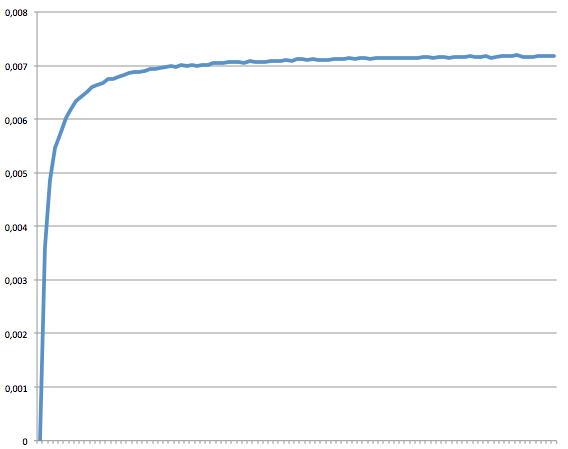
\includegraphics[height=0.5\textheight, width=0.8\textwidth]{D.png}
\end{center}
когда мы получаем реализацию дисперсии, то находимся где-то на этом графике, но ведем себя так как будто в бесконечности.
\end{frame}

\begin{frame}{Akaike information criterion}
\small
Будем считать, что мы знаем истинную функцию распределения $h_0$, тогда, мы можем посчитать $KL(h_0 \| \hat{h})$ для любого решения $\hat{h}$. Понятно, что $h_0$ на практике неизвестно, но оказывается сравнить $KL(h_0 \| \hat{h})$ мы все равно можем (Akaike (1974)):
$$AIC(h, y, X) = 2d(h) - 2 LL(y|X,h)$$
Где $d$ --- мера сложности решения. Например в линейных $d = \|\beta\|_0$. Закон асимптотический, поэтому можно применять только для больших $|X|$. Используют также:
$$
AICc(h, y, X) = AIC(h,y,X) + \frac{2d(h)(d(h) + 1)}{|X| - d(h) - 1}
$$
\end{frame}

\subsection{Про что мы умолчали}
\begin{frame}{Какие еще подходы бывают}
\begin{itemize}
  \item Co-clustering
  \item Байесова модель поведения пользователя
  \item Ближайшие соседи  
\end{itemize}
\end{frame}

\subsection{Factorization machines} % Статья http://www.ismll.uni-hildesheim.de/pub/pdfs/Rendle2010FM.pdf

\begin{frame}{Другой подход к построению модельной матрицы}
Последние много слайдов мы решали задачу регрессии. Давайте это прямо и напишем
\begin{center}
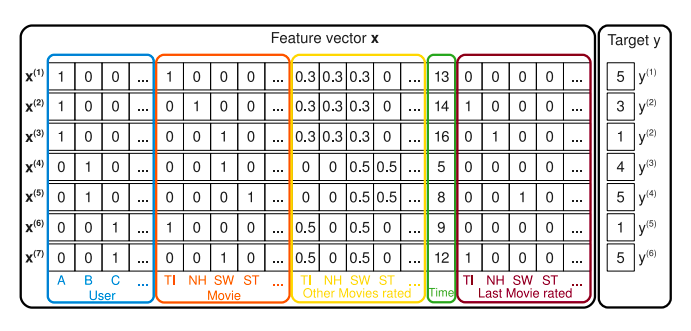
\includegraphics[width=1\textwidth]{FMSetup.png}
\end{center}
\end{frame}

\begin{frame}{Factorization machine}
\small
$$
h(x, \beta) = \beta_0^0 + \sum_i \beta_i^1 x_i + \sum_i \sum_{j > i} (\beta_i^2, \beta_j^2)x_i x_j
$$
и найдем
$$
\arg \min_\beta \|h(X, \beta) - y\|_2
$$
Такая постановка называется Factorization Machine (FM) второго порядка.
\end{frame}

\subsection{Проблема холодного старта}
\begin{frame}{Проблема холодного старта}
Что делать с новыми пользователями, история по которым неизвестна?
\begin{itemize}
  \item Посмотреть на ``средних'' (да-да, порекомендуйте мне Верку Сердючку!)
  \item Узнать хоть что-то про пользователя (регион, IP, откуда пришел (реферер), время захода, etc.) и построить правильный prior.
\end{itemize}
\end{frame}

\begin{frame}{Что мы сегодня узнали I}
\small
Про SVM
\begin{itemize}
  \item SVM можно делать в случае линейной неразделимости
  \item Формулы получаются почти такие же, но еще и с верхней границей на $\lambda$
  \item В SVM есть ядра, их можно подбирать, однако решение в этом случае включает все граничные точки из-за того, что $\Psi$ не определено в явном виде
  \item SVM можно рассматривать как минимизацию hindgу loss с регуляризацией по Тихонову
\end{itemize}
И не только:
\begin{itemize}
  \item На ядрах можно делать не только SVM, но и регрессию
  \item Несколько способов построения мультиклассификатора и их обобщение
\end{itemize}
\end{frame}

\begin{frame}{Что мы сегодня узнали II}
\small
Про CF:
\begin{itemize}
  \item Есть такая задача
  \item Ее можно решать просто и непросто
  \item Задачу CF можно свести к линейной регрессии с регуляризацией, и это работает
  \item Наиболее эффективный из известных мне методов CF (FM)
\end{itemize}
И не только:
\begin{itemize}
  \item Бывают регуляризации, построенные по принципу скорректированных оценок
\end{itemize}
\end{frame}

\end{document}
